\documentclass[12pt]{ociamthesis}  % default square logo 
%\documentclass[12pt,beltcrest]{ociamthesis} % use old belt crest logo
%\documentclass[12pt,shieldcrest]{ociamthesis} % use older shield crest logo

%load any additional packages
\usepackage{amssymb}
\usepackage{amsmath}
\usepackage{listings}
\usepackage{textcomp}

\lstset{language=Scala, upquote=true}
%input macros (i.e. write your own macros file called mymacros.tex 
%and uncomment the next line)
%\include{mymacros}

%My shortcuts:
\newcommand{\R}{\mathcal{R}}
\newcommand{\K}{\mathbf{K}}
\newcommand{\coll}[2]{#1 \rightarrow #2}
\newcommand{\prim}[1]{\textrm{\textit{#1}}}
\newcommand{\OR}{\: | \:}
\newcommand{\Bag}[1]{\prim{Bag}[#1]}
\newcommand{\For}[2]{\textrm{for}(#1 \leftarrow #2)}
\newcommand{\If}[1]{\textrm{ if #1}}
\newcommand{\ForIf}[3]{\For{#1}{#2 \If #3}}
\newcommand{\Yield}[1]{\textrm{ yield } #1}
\newcommand{\YieldP}[2]{\Yield #1 \mapsto #2}
\newcommand{\Collect}[1]{\textrm{ collect } #1}
\newcommand{\proj}[2]{#1.\_#2}
\newcommand{\pair}[2]{\langle #1, #2 \rangle}
\newcommand{\Label}{\prim{Label}}
\newcommand{\String}{\prim{String}}
\newcommand{\Int}{\prim{Int}}
\newcommand{\Unit}{\prim{Unit}}
\newcommand{\vs}{\vspace{1em}}
\title{Efficient Processing of Nested Collections in Apache Spark}   %note \\[1ex] is a line break in the title

\author{Theodore Dickson}         %your name
\college{Worcester College}  %your college

%\renewcommand{\submittedtext}{change the default text here if needed}
\degree{MSc in Computer Science}     %the degree
\degreedate{September 2018}         %the degree date

%end the preamble and start the document
\begin{document}

%this baselineskip gives sufficient line spacing for an examiner to easily
%markup the thesis with comments
\baselineskip=18pt plus1pt

%set the number of sectioning levels that get number and appear in the contents
\setcounter{secnumdepth}{3}
\setcounter{tocdepth}{3}


\maketitle                  % create a title page from the preamble info
%%\begin{dedication}
This thesis is dedicated to\\
 someone\\
for some special reason\\
\end{dedication}        % include a dedication.tex file
%%\begin{acknowledgements}
plenty of waffle, plenty of waffle, plenty of waffle, plenty of waffle,
plenty of waffle, plenty of waffle, plenty of waffle, plenty of waffle.
\end{acknowledgements}   % include an acknowledgements.tex file
\begin{abstract}
Apache Spark is a parallel data processing framework with a generic collection API, allowing the distributed processing of any serialisable datatype. Though this allows the construction and processing of nested collections, severe performance issues are encountered when these nested collections exhibit skew due to the inability to distribute them among multiple worker nodes. Further, many nested queries are unable to be incrementalised efficiently. Attempts to rectify this often involve a technique called shredding, which decouples the nested collections from the main query and allows them to be distributed and updated separately. However, many of the shredding transformations proposed have limited scope in the queries to which they can be applied, and are not offered as programmatic tools which can automatically transform queries.

In this work we develop a variant of the Nested Relational Calculus (NRC) which supports a compositional and generic shredding transformation. We implement it with a Scala DSL, which allows NRC queries to be expressed with natural and minimal syntax. The DSL can shred and evaluate queries on local Scala collections, Spark RDDs and Spark DStreams, and is easily extensible to other data types. We also contribute several novel techniques for developing DSLs in Scala which are generally applicable to many similar tasks.

We obtain performance gains of up to $5.5\times$ on shredded queries on Spark DStreams, although not all queries are sped up by shredding. We conclude that while shredding shows promise and this work contributes greatly to the ease of implementing such query transformations, further work would be necessary in order to enable shredding to be a worthwhile optimisation to integrate with Spark or other data processing frameworks.  
\end{abstract}          % include the abstract

\begin{romanpages}          % start roman page numbering
\tableofcontents            % generate and include a table of contents
%%\listoffigures              % generate and include a list of figures
\end{romanpages}            % end roman page numbering

%now include the files of latex for each of the chapters etc
\chapter{Introduction}

\section{Problem statement} {

Apache Spark \cite{spark} is an open-source framework for in-memory distributed processing of data sets. Since its initial release in 2014 it has quickly become one of the most popular frameworks for large-scale data analysis, owing largely to its user-friendly functional APIs (offered in Scala, Python, R and SQL) and impressive out-of-the-box performance. A number of domain-specific libraries (such as for machine learning and graph processing) have further enabled its wide adoption in industry.

Although Spark can transform collections of arbitrary types, it can exhibit severe performance problems when processing nested data (i.e. data with inner collections). Data of this type is commonplace, for example nested formats such as JSON and XML, or graphs in the adjacency list format. In particular, distributed processing of such data where the nested collections have skewed cardinalities leads to load imbalance amongst the machines in the cluster. At best, load imbalance causes inefficient use of resources. At worst, machines with the heaviest loads can run out of memory, causing slowdowns when results spill to the disk, and eventually total program failure when disk space runs out as well. Crucially, heavily skewed data is surprisingly common, owing to the power-law dynamics which govern many naturally occurring phenomena, especially social networks and other graph-like structures.

Additionally, although Spark offers powerful abstractions for processing streamed data, many queries involving nested collections do not incrementalise well. That is to say, it is not possible to process only the new batch and update the output with the latest result. Instead, with each new batch of data in the stream, the entire output must be recomputed.

Spark unfortunately does not offer any tools to deal with these performance issues. Instead, users must manually rewrite affected queries in order to flatten their inputs and/or outputs. However, this process is time-consuming and error prone, not least because many datasets are more naturally reasoned about as containing nested collections. The popularity of the aforementioned nested data formats is testament to this.

}

\section{Motivating example} {

To demonstrate this issue, let us consider the following scenario. A streaming music service allows listeners to rate tracks as they listen to them, with either a like (+1) or a dislike (-1). These ratings are stored using the following structure of case classes:

\begin{lstlisting}

case class Rating(artist: Artist, track: Track, value: Int)
case class Artist(id: Long, name: String)
case class Track(id: Long,  title: String)

\end{lstlisting}

The full dataset can therefore be processed in Spark via an \lstinline{RDD[Rating]}. The streaming service wishes to calculate for each artist, the set of their tracks that have been rated in the past day and for each track its aggregate rating. They wish to store this data in nested form so that it can efficiently provide the results for an endpoint in the service's public API which provides these track ratings for requested artists. Therefore they wish to calculate this result as an \lstinline{RDD[(Artist,Map[Track,Int])]}. 

The following spark query is the standard way to compute this:

\begin{lstlisting}

val ratings: RDD[Rating] //the input set of ratings
val trackRatingsByArtist: RDD[(Artist,Map[Track,Int])] =
  rating.groupBy(_.artist) //group by artist
    .map { case (artist,ratings) => //for each artist
      (artist, //return the artist
       ratings.map { case Rating(_,track,value) => (track,value) } 
        .reduceByKey(_ + _)
	.toMap //and aggregate the total ratings for each track
	)
    }

\end{lstlisting}

Firstly, this query is likely to exhibit severe load-balancing issues. Since a small number of artists are likely to represent a large proportion of ratings, the initial \lstinline{groupBy} in the query will likely create an extremely skewed \lstinline{RDD} by collecting every rating for a given artist into the same row. 

Secondly, this query cannot be \textit{efficiently incrementalised}. This means that its results cannot be updated with an efficient \textit{union} operation, given a new batch of data, without reprocessing the original output in any way. To demonstrate this, suppose that the music service instead wishes to calculate an up-to-date version of this dataset every hour, by processing an \lstinline{RDD} of the ratings for the last hour and combining this with the previous version. That is, we have:

\begin{lstlisting}
val oldTrackRatingsByArtist: RDD[(Artist,Map[Track,Int])]
val ratingsDelta: RDD[Rating]
\end{lstlisting} 

and then calculate the above query \textit{trackRatingsByArtist} just for the latest ratings:

\begin{lstlisting}
val trackRatingsByArtistDelta: RDD[(Artist,Map[Track,Int])]
\end{lstlisting}

Then the RDD:

\begin{lstlisting}
val oldTrackRatingsByArtist.union(trackRatingsByArtistDelta)
\end{lstlisting}

is not the correctly up-to-date version. It will include duplicate entries for each artist appearing in both the old version and the latest ratings. 

}

\section{Shredding} {

Our approach is to transform such queries using a process called \textit{shredding}, which solves the two root causes of the problem. First, that Spark only parallelises processing at the top-level, and has no mechanism for distributing inner collections, which is the cause of load imbalance.  Second, that the construction of nested collections does not benefit from the algebraic property of distributivity, as we will see in section \cite{}, which is what prevents efficient incrementalisation.

Shredding does this by pinpointing the places in a query in which nested collections are constructed, and instead replacing them by unique defining labels. Hence, the principal output of a shredded query is flat, i.e. it contains no nested collections. Along with the flat output, the shredding transformation additionally produces a shredding context. This is a set of queries which compute the dictionaries defining the inner collections associated to each label. These dictionaries are implemented in such a way that the definitions of the labels can in fact be distributed as well as efficiently updated.

In our simple example above, the principal output would be an \lstinline{RDD[(Artist,Label)]} and the shredding context would contain a corresponding \lstinline{Dictionary[Label,Map[String,Int]]}. (We leave discussion of the implementation of the dictionary for later).

However, this shredded output comes with a tradeoff. When the nested collections defined by the dictionaries are needed, there is a cost to looking them up. Whether the tradeoff is beneficial overall will depend on how the structure of the input data, the type of query and how the output is consumed. In data with only minor skew, the lookup cost may not be worth a relatively small load-balancing benefit, whereas when the skew is more severe, it is more likely to have a measurable performance benefit.

It will also depend on whether the entire nested output is needed or just a small part. In the in the music service scenario for example, if each API request only needs the nested output for a small number of artists, the lookup costs in the system will be very small compared to the load-balancing benefits.

With regard to incrementalised (or streamed) queries, the benefit of this tradeoff will be highly dependent on how frequently the output is consumed. For example, if the query is consumed very infrequently compared to how often it is updated, the more efficient updates may counteract even a very high lookup cost.

\subsection{Related work} {}

\subsection{Automating shredding} {
In this work, we use a variant of the shredding transformation introduced in \cite{draftpaper}, which operates on queries written in variant of the Nested Relation Calculus (NRC). While it was shown that certain shredded queries can be processed up to 21.9x faster, the shredding transformation was applied manually. Although this demonstrated the validity of the approach, and provided a strict algorithmic process for manual query-rewriting, it does not truly solve the problem.

Therefore our goal is to implement the automatic shredding of queries without sacrificing the performance benefits demonstrated in \cite{draftpaper}. We aim to do this by providing a domain-specific language (DSL) in which users can express NRC queries with natural syntax, and then automatically evaluate them in Spark using the shredding transformation.
}

}


\section{Contributions} {
The main contributions of this work are as follows:

\begin{itemize}
\item{We provide a Scala DSL which allows users to easily write NRC queries with natural syntax. Queries written in this way can be automatically evaluated, with or without the shredding transformation applied, with the full runtime safety guarantees of the Scala compiler.}
\item{This DSL works with both local collections and Spark collections, and is easily extensible to other frameworks thanks to a clean, modular design based largely on the typeclass pattern.}
\item{We introduce an updated version of the NRC which enabled the automatic evaluation of queries in Spark, by replacing constructs which proved hard to translate to valid Spark code.}
\item{\textit{(summary of performance benefits)}}
\end{itemize}
}

\section{Structure of the text} {
The rest of the report proceeds as follows. In the first chapter, we introduce the variant of the NRC used in this work, and define the shredding transformation on queries written in this calculus. In the second chapter, we describe the basic implementation of the DSL - both how an appropriate representation for queries was designed and how various features of Scala allowed these queries to be generated with user-friendly syntax. In chapter 3, we demonstrate how the evaluation of these queries was achieved, both with and without shredding.  In chapter 4, we show how we extended the DSL to incrementally evaluate queries. In chapter 5 we provide some experimental results and discuss their significance. Finally, we provide some concluding remarks including possible directions for future work.
}
\chapter{Nested Relational Calculus} \label{nrc}

In this chapter we explain the variant of the nested relational calculus used in this work.
First we explain how its semantics allow arbitrary nesting of collections, and introduce the core algebraic operators, showing how they enable a wide range of queries. Then we introduce some syntactic constructions which allow us to more naturally express nested queries. We explain the two forms that nested queries can take (key-nested and value-nested), and why the former is preferable semantically but not efficiently parallelised or incrementalised. Next we introduce the delta expressions for each operator, and show that while most operators incrementalise efficiently due to their algebraic properties, others must be recomputed with each update. Finally we provide a full description of the shredding transformation, and show how it allows us to simulate the semantics of a single key-nested query with a set of value-nested queries, thus retaining the performance benefits of value-nesting.


\section{Type system} {

In order to apply the shredding operation outlined in the previous chapter, we introduce a variant of the nested relational calculus which uses \textit{generalised multiset semantics}. As opposed to a regular multiset, or \textit{bag}, in which each element in a set is associated with an integer value, in our generalised multiset semantics we model collections by mappings $ \coll{\K}{\R} $ where values can be of any type which admits a ring structure $ (\R,0_\R,+_\R,-_\R,1_\R,*_\R) $. In the following we will show the two key properties of these semantics. Firstly, that they admit nesting of collections to arbitrary depth, and secondly, that they give rise to the potential for efficient incrementalisation and parallelisation since the majority of the operators we will introduce are distributive ring operations.

Figure \ref{nrctypes} formally describes the type system that enables these semantics, using an inductive definition.

\begin{figure}
\begin{equation*}
\begin{aligned}
\R := \prim{Int} \OR \prim{Bool} \OR \R \times  \R \OR \coll{\K}{\R} \\
\K := \prim{Dom} \OR  [\R]  \OR \prim{Label} \\
\end{aligned}
\qquad
\begin{aligned}
\end{aligned}
\end{equation*}
\caption{The type system of the NRC}
\label{nrctypes}
\end{figure}

It will also be useful to introduce the notation $\Bag{\K} := \coll{\K}{\prim{Int}}$, for collections with integer multiplicity.

\subsection{Ring types} {
The base cases of our ring type are the integers and the booleans. Integers admit the ring structure $(\mathbb{Z},0,+,-,1,*)$, and booleans the structure $(\mathbb{B}, false,OR,NOT,true,AND)$. Note that it is trivial to extend this calculus to other primitive types admitting a ring structure, such as the real numbers, but for brevity we omit these. 

The first of our inductive cases is the product type $\R \times \R$. A product of two ring types $\R_1$ and $\R_2$ trivially admits a ring structure by pairing the 0 and 1 elements and applying the operations of $\R_1$ and $\R_2$ element-wise. Although in practice we will be able to use tuples of any arity, in this formalism we only define operations for a pair, as higher arities are isomorphic to nesting products within the second element.

The second and crucial inductive case is the collection type $\coll{\K}{\R}$, which itself admits a ring structure in which $\R$'s operations are applied element-wise over the key space $\K$. For example, if we have two collections $X: \coll{\K}{\R}$ and $Y: \coll{\K}{\R}$ then:

\begin{equation*}
\begin{split}
& (X+Y)(k)  = X(k) +_\R Y(k) \\
& (X*Y)(k) = X(k) *_\R Y(k)
\end{split}
\end{equation*}

If $\R$ is an $\prim{Int}$, so that $X,Y: \Bag{\K}$, then we can see that $+$ corresponds to bag union. We can also see that $*$ is join-like - a key will only have non-zero value in the resulting collection if it has non-zero value in each of $X$ and $Y$.

In this way, we can use collections themselves as multiplicities. For example, a collection of type $\coll{\K_1}{(\coll{\K_2}{\R})}$ associates a collection of type $\coll{\K_2}{\R}$ to each key of type ${\K_1}$. This is what we call \textit{value} or \textit{ring} nesting and is the first way to obtain nested collections.

\subsection{Key types} {

For keys, the base types are the $\prim{Dom}$ types. These are the types of the active domain of the database. When using Apache Spark for example, this constitutes all serializable Scala data types. In a typical relational database this would be much more restricted, to types such as INT, FLOAT, VARCHAR, TIMESTAMP, and so on. 

The type $[\R]$ (the boxed ring type) offers ring types for use as keys while retaining the view of their ring structure, thus marking the places where shredding can be performed. For example, a collection of type $\coll{(\K_1,[\coll{\K_2}{\R}])}{\prim{Int}}$ maps a pair of two key types, $\K_1$ and the boxed ring type, $[\coll{\K_2}{\R}]$ to a multiplicity of $\prim{Int}$ type. This is what we call \textit{key nesting}. 

The $\prim{Label}$ type represents places we have applied shredding, in order to replace key-nested collections with labels. For example, in a query which produces a result of type  $\coll{(\K_1,[\coll{\K_2}{\R}])}{\prim{Int}}$, we would expect shredding to instead produce a result of type 
$\coll{(\K_1,\prim{Label})}{\prim{Int}}$, along with a dictionary of type $\coll{\prim{Label}}{(\coll{\K_2}{\R})}$. Note that both of these types do not contain key-nested collections. Instead our dictionary uses value-nesting. This will be crucial to how we efficiently incrementalise such shredded queries.

}

\section{Expressions}

\begin{figure}
\begin{equation*}
\begin{split}
k := \ & c \OR x \OR \langle k_1, k_2 \rangle \OR \proj{k}{i} \\ \\
r := \ & c \OR X \OR \langle r_1, r_2 \rangle \OR \proj{r}{i} \OR \\
& r_1 + r_2 \OR -r \OR r_1 \ast r_2 \OR r_1 \cdot r_2 \OR \\
& join(r_1,r_2) \OR sum(r) \OR p(k) \OR \\
& sng(k,r) \OR \{ x => r \} \OR group(r)
\end{split}
\end{equation*}
\caption{Valid expressions in the NRC.}
\label{nrcexprs}
\end{figure}

Figure \ref{nrcexprs} introduces the constructions that define the valid expressions in our calculus. In this section we explain these and discuss their algebraic properties.

\subsection{Ring expressions} {
The base expressions of ring type are constants and input collections, denoted by $c$ and $X$ respectively. Constants will be of $\prim{Int}$ or $\prim{Bool}$ type in this restricted formalism, but in practice can be of any numeric type or other primitive type admitting a ring structure. Input collections are datasets of type $\coll{\K}{\R}$, where $\K$ is any valid key type and $\R$ any valid ring type. For example, in our motivating example, the input collection \textit{ratings} is of type $\coll{(Artist \times Track)}{\prim{Int}}$. We also have a standard tupling operator denoted by $\langle , \rangle$ and can project such product types using the notation $\proj{r}{i}$.

Next we have $+$, $-$, and $\ast$, the algebraic operators defined by the ring structure of $\R$. It will be important when discussing incrementalisation and parallelisation to note that  $\ast$ is distributive with respect to $+$:
\[
a*(b + c) = a*b + a*c.
\]

The dot product ($\cdot$) is a generalised multiplication operator which accepts any two arguments of ring type. It is defined using $*$ as follows:
\begin{equation*}
\begin{split}
& \textrm{If } X: \prim{Int}, \ Y: \prim{Int}\textrm{, then } X \cdot Y = X * Y \\ \\
& \textrm{If } X: \coll{\K}{\R}, \ Y: \prim{Int}\textrm{, then } X \cdot Y : \coll{\K}{\R \cdot \prim{Int}}, \\
& (X \cdot Y)(k) = X(k) \cdot Y\textrm{, for all }k: \K \\ \\
& \textrm{If } X: \coll{\K_1}{\R_1}, \ Y: \coll{\K_2}{\R_2}\textrm{, then } X \cdot Y : \coll{\langle \K_1, \K_2 \rangle}{\R_1 \cdot \R_2} \\
& (X \cdot Y)(\langle k_1, k_2 \rangle) = X(k_1) \cdot Y(k_2)\textrm{, for all }k_1,k_2: \K
\end{split}
\end{equation*}
This operation can natively implement certain useful operations. For example, the dot product of $\Bag{\K_1}$ and $\Bag{\K_2}$ produces their cartesian product.

The dot product is distributive:
\vs\begin{equation*}
\begin{split}
& \textrm{If } X: \prim{Int}, \ Y: \prim{Int}\textrm, \ Z: \Int: \\
&X \cdot (Y + Z) = X * (Y + Z) = X*Y + X*Z = X \cdot Y + X \cdot Z \\ \\
& \textrm{If } X: \coll{\K}{\R}, \ Y: \prim{Int}, \ Z: \Int: \\
& (X \cdot (Y+Z))(k) = X(k) \cdot (Y+Z) = X(k) \cdot Y + X(k) \cdot Z = (X \cdot Y)(k) + (X \cdot Z)(k) \\ \\
& \textrm{If } X: \coll{\K_1}{\R_1}, \ Y: \coll{\K_2}{\R_2}, \ Z: \coll{\K_2}{\R_2} \\
& (X \cdot (Y+Z))(\langle k_1, k_2 \rangle) = X(k_1) \cdot (Y+Z)(k_2) = X(k_1) \cdot Y(K_2) + X(k_1) \cdot Z(k_2) \\
&= (X \cdot Y)(k_1) + (X \cdot Z)(k_2) 
\end{split}
\end{equation*}
It also allows us to extend the native ring multiplication operation to collections of the same key type but differing ring types, by defining the output value of each key as the dot product of the values of the key in each input collection:
\begin{equation*}
\begin{split}
& X: \coll{\K}{\R_1}, \ Y: \coll{\K}{\R_2} \\
& X * Y : \coll{\K}{\R_1 \cdot \R_2} \\
& (X*Y)(k) = X(k) \cdot Y(k)
\end{split}
\end{equation*}
We will see how this extension to multiplication allows us to define a for-comprehension construct with very natural semantics.

Note that when applied to collections, $*$ operator can be described as join-like. This is because a key will only be present (i.e. have non-zero value) in the output collection if it has non-zero value in both of the input collections. However, since it performs this join on the entire key, it is not general enough to model many useful joins. Thus we introduce a separate join operator, which only operates on collections, and joins only on the first element of a product-typed key. It is defined as follows:
\begin{equation*}
\begin{split}
& X: \coll{(\K,\K_1)}{\R_1},  Y: \coll{(\K,\K_2)}{\R_2} \\
& join(X, Y): \coll{(\K, (\K_1,\K_2))}{\R_1 \cdot \R_2} \\
& join(X, Y)(\langle k, \langle k_1, k_2 \rangle \rangle) = X(\langle k, k_1 \rangle) \cdot Y(\langle k, k_2 \rangle)
\end{split}
\end{equation*}
We can see that this is a join as a key $\langle k, \langle k_1, k_2 \rangle \rangle$ will only be non-zero in the output if $\langle k, k_1 \rangle$ is non-zero in $X$ and $\langle k, k_1 \rangle$ is non-zero in $Y$. It is general enough to model all inner joins if we re-order the elements (or columns) of the key such that the element(s) we wish to join on constitute the first element of the key and the other columns are nested within the second element. 

\noindent The $join$ operator is also distributive:
\begin{equation*}
\begin{split}
&X: \coll{(\K,\K_1)}{\R_1},  \ Y: \coll{(\K,\K_2)}{\R_2}, \ Z: \coll{(\K,\K_2)}{\R_2} \\
&join(X,Y+Z)(\pair{k}{\pair{k_1}{k_2}}) = X(\pair{k}{k_1}) \cdot (Y+Z)(\pair{k}{k_2}) \\
&=X(\pair{k}{k_1}) \cdot Y(\pair{k}{k_2}) + X(\pair{k}{k_1}) \cdot Z(\pair{k}{k_2}) \\
&=join(X,Y)(\pair{k}{\pair{k_1}{k_2}}) + join(X,Z)(\pair{k}{\pair{k_1}{k_2}})
\end{split}
\end{equation*}

The sum operator is another which will be used in the for-comprehension construct, and is defined as follows: 
\begin{equation*}
\begin{split}
 & X: \coll{\K}{\R} \\
 & sum(X): \R \\
 & sum(X) = \sum_{k: K} X(k)
\end{split}
\end{equation*}
It is only defined for collection types, and, for example, when applied to a bag returns its aggregate count.
 
\vs The predicate operator $p(k)$ encapsulates any function accepting a key and returning a boolean. We will see how it enables us to do things such as filter collections.
 
\vs The \textit{singleton} constructor is $sng$. With $k: \K$ and $r: \R$, $sng(k,r)$ constructs a collection of type $\coll{\K}{\R}$ with the single element $k  \mapsto r$. We will see how this combines with our for-comprehension construct to create nested collections.
 
\vs The infinite mapping $\{x => r\}$ allows us to express functions from key types to value types as collections of infinite domain, where the key is a variable expression $x$ and the value is a ring expression $r$ which may use the variables introduced in $x$. When such an expression is multiplied with a finite collection, the variable expression is bound to each of the keys in the finite collection in order to produce a concrete result.

The following example shows us how this allows transformations of finite collections:

\noindent Let $k_1,k_2: K$ be variables. Let $X: \Bag{\K \times \K}$. Let $p(\langle k_1, k_2 \rangle) = k_1 == k_2$ be the predicate comparing $k_1$ and $k_2$ for equality. \\
Let $Y = X * \{\langle k_1, k_2 \rangle => p(\langle k_1, k_2 \rangle)\}$. \\ Applying the definition of *, and assuming $k_1,k_2$ are in the domain of $X$: \\
\begin{equation*}
\begin{split}
Y(\langle k_1, k_2 \rangle) &= X(\pair{k_1}{k_2}) \cdot 1 = X(\pair{k_1}{k_2})\textrm{, if } k_1 == k_2 \\
&= X(\pair{k_1}{k_2}) \cdot 0 = 0\textrm{, otherwise}
\end{split}
\end{equation*}
Hence $Y$ is X filtered to only those keys whose first and second elements are equal.

\vs The last ring-typed construct is group, and is the operator which constructs key-nested collections. It is defined on collections with keys of pair type, as follows:
\begin{equation*}
\begin{split}
&X: \coll{\K_1 \times \K_2}{\R} \\
&group(X): \coll{\K_1 \times [\coll{\K_2}{\R}]}{\prim{Bool}} \\
&group(X)(\pair{k_1}{k_2'}) = true \iff k_2' = \sum_{(\pair{k_1'}{k_2} \mapsto r) \in X : \ k_1' = k_1} {\{k_2 \mapsto r\}} 
\end{split}
\end{equation*}
This creates a key in the output for each unique first element of the key in the input. These keys are paired with the boxed collection of all of the second elements they appear with in the input. In this way it is a grouping of the input by the first element of the key. For example:
\begin{equation*}
\begin{split}
&X: \Bag{\prim{String}\times \prim{String}} \\
&X = \{(a,b) \mapsto 1, (a, c) \mapsto 2, (b,d) \mapsto 3\} \\
&group(X) = \{\langle a, \{b \mapsto 1, c \mapsto 2\} \rangle \mapsto true, \langle b, \{d \mapsto 3 \} \rangle \mapsto true \}
\end{split}
\end{equation*}
While this boolean value may seem redundant, and thus this representation may seem to offer no benefit over the value-nested representation $\coll{\K_1}{(\coll{\K_2}{R})}$, it actually offers a key semantic benefit. It allows us to keep track of values of type $\K_1$ whose nested collections become empty when updating inputs to a query. Using the example above, suppose we receive an update to $X$:
\begin{equation*}
\dX = \{(\pair{b}{d} \mapsto -3\}
\end{equation*}
This translates to updating the key-nested collection $\pair{b}{\{d \mapsto 3\}}$:
\begin{equation*}
 \pair{b}{\{d \mapsto -3, d \mapsto 3\}} = \pair{b}{\{\}}
 \end{equation*}
However the entry $\pair{b}{\{\}} \mapsto true$ remains in the output, indicating that the inner collection keyed by $b$ exists but is empty.
Letting $group^v(X)$ be the value-nested representation of $group(X)$:
\begin{equation*}
group^v(X) = \{a \mapsto \{b \mapsto 1, c  \mapsto 2\}, b \mapsto \{d \mapsto 3\}\}
\end{equation*}
When we update this with $\{b \mapsto \{d \mapsto 3\}\}$, we get:
\begin{equation*}
group^v(X) = \{a \mapsto \{b \mapsto 1, c  \mapsto 2\}, b \mapsto \{d \mapsto 0\}\} = \{a \mapsto \{b \mapsto 1, c  \mapsto 2\}\}
\end{equation*}
And so $b$ disappears from the top-level of our output entirely. 

\subsection{Key expressions} {
The base key expressions are either constants, denoted $c$, or variables, denoted $x$, which are strictly those introduced as the keys of an infinite mapping. As with ring expressions, we also have tupling and projection. 
}

\section{For-comprehension syntax} {
In this section we introduce several variants of a familiar syntactic construction, the for-comprehension, which will allow many queries to be written more naturally.

Let $X$ be a finite collection of type $\coll{\K}{\R}$, $r_1$ be a ring expression of type $\R_1$, and $x$ be a variable of type $\K$. Our basic for-comprehension syntax is thus defined as:
\begin{equation*}
\For{x}{X} \Collect{r_1} := sum(X * \{x => r_1\})
\end{equation*}
It is helpful to think of this as iterating over the key-value pairs $\pair{k}{r}$ in $X$, calculating the value of $r_1$ for each key $k$, and aggregating the result of multiplying this with $r$. For example, with $X: \Bag{\Int}$, the query:
\begin{equation*} 
\For{x}{X} \Collect{x > 2} = sum(X * \{x => x > 2\})
\end{equation*}
calculates the aggregate count of the keys in $X$ which are greater than 2, since:
\begin{equation*}
\begin{split}
(X*\{x => x > 2\})(y) &= X(y)*true = X(y)\textrm{, if } y > 2 \\
 &= X(y)*false = 0\textrm{, otherwise.}
\end{split}
\end{equation*}
We now add a variant of this which enables filtering collections with a natural syntax. With $p(x)$ a predicate expression:
\begin{equation*}
\ForIf{x}{X}{p(x)} \Collect{x > 2} := sum(X * \{x => r_1 \cdot p(x) \})
\end{equation*}
Hence, we can instead write the above query as:
\begin{equation*}
\begin{split}
\ForIf{x}{X}{x > 2} \Collect{1} &= sum(X * \{x => 1 \cdot (x > 2) \}) \\
&=sum(X * \{x => x > 2) \}
\end{split}
\end{equation*}
These examples are quite limited in that they are only aggregations of a collection $X$. In order to transform $X$ more generally, we can use the singleton constructor. For example, consider the following query:
\begin{equation*}
\begin{split}
&X: \coll{\K_1 \times \K_2}{\R} \\
&Y = \For{\pair{k_1}{k_2}}{X} \Collect{sng(\pair{k_2}{k_1}, 1)}
\end{split}
\end{equation*}
Then $Y$ is $X$ but with the pairs reversed. To see how this works, let's examine the translation of $Y$ into basic syntax: 
\[ Y = sum(X*\{\pair{k_1}{k_2} => sng(\pair{k_2}{k_1},1)\}) \]
The inner expression $X*\{\pair{k_1}{k_2} => sng(\pair{k_2}{k_1},1)\}$ iterates over $X$ and and maps each key $\pair{k_1}{k_2}$ to its original value, multiplied by $sng(\pair{k_2}{k_1},1)$. Thus, suppose $X = \{\pair{a}{b} \mapsto 1, \pair{c}{d} \mapsto 2\}$, then:
\begin{equation*}
X*\{\pair{k_1}{k_2} => sng(\pair{k_2}{k_1},1)\} = \{(a,b) \mapsto \{(b,a) \mapsto 1\}, (c,d) \mapsto \{(d,c) \mapsto 2\}\}
\end{equation*}
Then the sum outside this simply aggregates all of the values via bag union, to produce the single collection:
\begin{equation*}
\{(b,a) \mapsto 1, (d,c) \mapsto 2\}
\end{equation*}
Which is indeed $X$ with the elements of the keys reversed. We encapsulate this construct with the following variant of our for-comprehension: 
\begin{equation*}
\begin{split}
\ForIf{x}{X}{p(x)} \Yield{k \mapsto r} &:= \ForIf{x}{X}{p(x)} \Collect{sng(k,r)} \\
& \ = sum(X * \{x => sng(k,r \cdot p(x)) \})
\end{split}
\end{equation*}
The $r$ is optional and defaults to 1. Thus, we can write the above query to reverse the elements in a product-type key as:
\[\For{\pair{k_1}{k_2}}{X} \Yield{\pair{k_2}{k_1}}\]
This is clearly a very natural syntax with which to manipulate collections corresponding to similar syntax in many programming languages.
}

\section{Restricted construction of key-nested collections}
The $group$ operator is the only way in this calculus to construct key-nested collections. We recognise that this is quite restrictive. In fact, in \cite{draftpaper}, the variant of the NRC used does not include this construct, but instead uses a more general construct $toK$ which boxes arbitrary sub-queries of ring type. Unfortunately, although this allows for a more general query language, the queries written in this way proved highly impractical to implement within Spark. For example, to express the grouping of a collection $X: \Bag{\K_1 \times \K_2}$ by the first element of the key, the following query would be used:
\begin{equation*}
\begin{split}
&\For{\pair{k_1}{k_2}}{X} \\
&\Yield{\pair{k_1}{toK(\ForIf{\pair{k_1'}{k_2'}}{X}{k_1 == k_1'} \Yield k_2')}}
\end{split}
\end{equation*}
Here, the logic to group is expressed by a nested iteration, filtered by a predicate to test for equality of the inner key with the outer key.
The naive way to implement the evaluation of such a query would lead to physically performing this nested iteration, which is clearly very inefficient compared to implementing it with a grouping primitive. Further, in Spark, nested iteration of RDDs is not supported at all.
Thus, without a dedicated optimiser to examine these queries and detect when nested iterations filtered by predicated correspond to grouping or other primitives, it is not possible evaluate such queries in Spark.

Hence it was decided to forego this operator in favour of the explicit $group$ operator which can be directly evaluated using the \lin{groupBy} method on an RDD, as we will see in Chapter \ref{evaluation}.
Despite this, we will see in Chapter \ref{results} that even with this restriction we are still able to express a wide range of quite complex queries. 

}

\section{Incremental updates to queries} { \label{deltas}

\begin{figure}
\begin{equation*}
\begin{aligned}
&\delta_X(c) = 0 \qquad \delta_X(X) = \Delta X \qquad \delta_X(Y) = 0\\
&\delta_X(\pair{r_1}{r_2}) = \pair{\delta_X(r_1)}{\delta_X(r_2)} \qquad \delta_X(\proj{r}{i}) = \proj{\delta_X(r)}{i}\\
&\delta_X(r_1 + r_2) = \delta_X(r_1) + \delta_X(r_2) \qquad \delta_X(-r) = -\delta_X(r)\\
&\delta_X(r_1 * r_2) = \delta_X(r_1)*r_2 + r_1*\delta_X(r_2) + \delta_X(r_1) * \delta_X(r_2) \\
&\delta_X(r_1 \cdot r_2) = \delta_X(r_1) \cdot r_2 + r_1 \cdot \delta_X(r_2) + \delta_X(r_1) \cdot \delta_X(r_2) \\
&\delta_X(join(r_1,r_2)) = join(\delta_X(r_1),r_2) + join(r_1,\delta_X(r_2)) + join(\delta_X(r_1),\delta_X(r_2)) \\
&\delta_X(sum(r)) = sum(\delta_X(r)) \qquad \delta_X(\{x => r\}) = \{x => \delta_X(r)\} \\
&\delta_X(sng(k,r)) = sng(e^{new},r)  + sng(e^{new},\delta_X(r)) - sng(e^{old},r) \\
&\delta_X(group(r)) = group(r + \delta_X(r)) - group(r)
\end{aligned}
\qquad
\end{equation*}
\caption{Delta derivation rules for NRC expressions.}
\label{deltaexprs}
\end{figure}

In this section we introduce \textit{delta expressions}, or expressions which compute the update to a query given an update to its inputs. For example, if we have some expression $r$ with an input collection $X$, and receive an update $\delta X$ for $X$ such that the new value of $X$ is $X^{new} = X + \delta X$, the delta expression $\delta_X(r)$ is some expression such that $r^{new}$ = $r + d_X(r)$.

Figure \ref{deltaexprs} shows these expressions. The fact that the updates are modelled with addition allows us to exploit the algebraic properties of the operators to derive efficient delta expressions in the majority of cases. For example, we exploit the linearity of $+$ to derive the delta rule:
\[\delta_X(r_1 + r_2) = \delta_X(r_1) + \delta_X(r_2)\]
since: 
\[r_1^{new} + r_2^{new} = (r1 + \delta_X(r_1)) + (r2 + \delta_X(r_2)) = (r_1 + r_2) + (\delta_X(r_1) + \delta_X(r_2))\]
Linearity is similarly used for $-$ and $sum$. These rules are efficient because they do not depend at all on $X$, only $\delta X$.

\vs The slightly more complicated rules for multiplication, the dot product, and the join operator are a result of their distributivity. We illustrate the derivation of the rule for multiplication below:
\begin{equation*}
\begin{split}
(r_1 + \delta_X(r_1))*(r_2 + \delta_X(r_2)) &= (r_1 + \delta_X(r_1))*r_2 + (r_1 + \delta_X(r_1))*\delta_X(r_2) \\
&= r_1*r_2 + \delta_X(r_1)*r_2 + r_1*\delta_X(r_2) + \delta_X(r_1) * \delta_X(r_2) \\
\implies \delta_X(r_1*r_2) &= \delta_X(r_1)*r_2 + r_1*\delta_X(r_2) + \delta_X(r_1) * \delta_X(r_2)
\end{split}
\end{equation*}
This derivation is also valid for the dot product and join operator as it only uses the distributive property which they all share. While these rules are not quite as efficient as the rules for the linear operators, they are still much more efficient than re-computing. This is because the terms that do depend on an input collection, e.g. $\delta_X(r_1) * r_2$, will constitute a join in practice between an update and only one of the input collections. Since the updates are in general small compared to the size of the input collections, these joins will be much more efficient that the cost of the original join between the two input collections.

\vs Unfortunately, we can see that the expressions for $sng$ and $group$ are not efficient - they do require recomputation. In the case of $sng$, this is because if the key-typed argument is affected by the update, the singleton collection must be fully reconstructed. However, if it is unaffected by the update, so that $e^{new} = e^{old} = e$, the delta expression simplifies as follows:
\begin{equation*}
\begin{split}
sng(e^{new},r) + sng(e^{new},\delta_X(r)) - sng(e^{old},r) &= sng(e,r) + sng(e,\delta_X(r)) - sng(e,r) \\
&= sng(e,\delta_X(r))
\end{split}
\end{equation*}
which is an efficient incrementalisation. In practice, usage of $sng$ will largely be confined to the for/yield construction where the yielded key is a variable expression, and so will be unaffected by updates to input collections. 

For $group$, this is because the construction of key-nested collections is fundamentally not distributive or linear. Thus, the only way to compute an updated output is to compute the updated input, apply $group$ to this, and substract the previous output. However, we will see in the next section how shredding removes the need for this recomputation by converting the construction of a key-nested collection into the construction of value-nested collection, which does indeed distribute over addition.
	
}

\section{The shredding transformation} {

In this section we define the shredding transformation. As previously described, when we shred a query, we produce both a flat version of the query, in which all key-nested collections have been replaced by labels, and the shredding context, a structure containing the dictionaries defining the labels appearing in the flat query. Therefore shredding consists of two separate transformations - the flattening of the query, which we will denote $(\cdot)^F$, and the derivation of the shredding context, which we will denote $(\cdot)^\Gamma$.

\subsection{Output type of the shredding transformation} {

It will be useful to first examine how shredding works at the type level. Figure \ref{shreddingtypes} defines the two output types of the two constituent transformations.

\begin{figure}
\begin{equation*}
\begin{aligned}[c]
&(\K_1 \times \K_2)^F : \K_1^F \times \K_2^F \\
&(\R_1 \times \R_2)^F : \R_1^F \times \R_2^F \\
&\prim{Int}^F : \prim{Int} \\
\\
&(\K_1 \times \K_2)^\Gamma : \K_1^\Gamma \times \K_2^\Gamma \\
&(\R_1 \times \R_2)^\Gamma : \R_1^\Gamma \times \R_2^\Gamma \\
&\prim{Int}^F : \prim{Unit} \\
\end{aligned}
\qquad
\begin{aligned}[c]
&(\coll{\K}{\R})^F : \coll{\K^F}{\R^F} \\
&[\R]^F: \prim{Label} \\
&\prim{Dom}^F : \prim{Dom} \\
\\
&(\coll{\K}{\R})^\Gamma : \K^\Gamma \times \R^\Gamma \\
&[R]^\Gamma : (\coll{\prim{Label}}{\R^F}) \times \R^\Gamma \\
&\prim{Dom}^\Gamma : \prim{Unit} \\
\end{aligned}
\end{equation*}
\caption{Output types of the shredding transformations.}
\label{shreddingtypes}
\end{figure}

The type returned by $(\cdot)^F$ is straightforward - it is recursively defined to simply replace all boxed ring types with the $Label$ type, and it does nothing to primitive types.

The type returned by of $(\cdot)^\Gamma$ slightly more complicated. The base cases of our primitive types contain no key-nested collections and so their context is empty, which is represented by the $\prim{Unit}$ type. Product types have a context consisting of the contexts of their elements, in a matching structure. Collections also have tupled shredding contexts, the first element for the context of it's key and the second for its value.

The interesting case is the boxed ring type $[\R]$. Here the shredding context will consist of two parts - first the dictionary defining the flattened boxed value, and second it recursively contains this value's shredding context. This represents the fact that shredding proceeds recursively - for a boxed collection $\coll{\K}{\R}$ either the key or the value may contain further key-nested collections and so it is shredded to produce the collection $\coll{\K^F}{\R^F}$ before producing the dictionary defining the inner labels. Otherwise, we would only be able to obtain the benefits of shredding for inner collections nested only at one level and not at arbitrary depth.

An important thing to note about these definitions is that the structure of the shredding context is fully defined by the type of the shredded query, and additionally mirrors the output type of the shredded query. This has two important benefits: Firstly, as we will show when defining the transformations themselves on our calculus constructs, this allows contexts to be combined when performing operations on shredded queries. For example, if we add two shredded queries, we need to element-wise perform union on their contexts. Secondly, it means that it is unambiguous as to which dictionary corresponds to which labels in the flat output.

To illustrate the process by which we apply the above rules to determine the flat output type and shredding context structure, we show an example of their application for a collection of type $\Bag{[\Bag{\prim{String}}]} = \coll{[\coll{\prim{String}}{\prim{Int}}]}{\prim{Int}}$:
\begin{equation*}
\begin{split}
(\coll{[\coll{\prim{String}}{\prim{Int}}]}{\prim{Int}})^F&: \coll{\Label}{\Int^F} \\
&: \coll{\Label}{\Int}
\end{split}
\end{equation*}
\begin{equation*}
\begin{split}
(\coll{[\coll{\prim{String}}{\prim{Int}}]}{\prim{Int}})^\Gamma&: ([\coll{\String}{\Int}]^\Gamma \times \Int^\Gamma) \\
&: (((\coll{\Label}{(\coll{\String}{\Int})) } \times (\coll{\String}{\Int})^\Gamma) \times \Unit) \\
&: (((\coll{\Label}{(\coll{\String}{\Int})) } \times (\String^\Gamma \times \Int^\Gamma) \times \Unit) \\
&: (((\coll{\Label}{(\coll{\String}{\Int})) } \times (\Unit \times \Unit) \times \Unit) \\
\end{split}
\end{equation*}

While in this simple example, the nested structure containing various empty contexts and only a single dictionary may seem unnecessary, in complex queries with many levels of nesting, there will be multiple dictionaries within the context and their location is determined by the inner collection they define, and so this type of structure is very useful.

}

\subsection{Formal definition of shredding}

\begin{figure}
\begin{equation*}
\begin{aligned}
&\pair{r_1}{r_2}^F = \pair{r_1^F}{r_2^F} \qquad (\proj{r}{i})^F = \proj{r^F}{i} \\
&(r_1 + r_2)^F = r_1^F + r_2^F \qquad (-r)^F = -(r^F) \\
&(r_1*r_2)^F = r_1^F * r_2^F \qquad (r_1 \cdot r_2)^F = r_1^F \cdot r_2^F  \\
&join(r_1,r_2)^F = join(r_1^F,r_2^F) \qquad sum(r)^F = sum(r^F) \\
&\{x => r\}^F = \{x => r^F \} \qquad sng(k,r)^F = sng(k^F,r^F) \\
&group(r)^F = flatGroup(r^F) \\
\end{aligned}
\qquad
\end{equation*}
\caption{Definition of $(\cdot)^F$ transformation.}
\label{flatdef}
\end{figure}

\begin{figure}
\begin{equation*}
\begin{aligned}
&\pair{r_1}{r_2}^\Gamma = \pair{r_1^\Gamma}{r_2^\G} \qquad (\proj{r}{i})^\G = \proj{r^\G}{i}  \qquad (p(x))^\Gamma = \emptyset \\
&(r_1 + r_2)^\G = r_1^\G \cup r_2^\G \qquad (-r)^\G = (r^\G) \\
&(r_1*r_2)^\G = r_1^\G \odot r_2^\G \qquad (r_1 \cdot r_2)^\G = \pair{r_1^{\G_1} \cap r_2^{\G_1}}{r_1^{\G_2} \odot r_2^{\G_2}}  \\
&join(r_1,r_2)^\G = \pair{\pair{r_1^{\G_{1_1}} \cap r_2^{\G_{1_1}}}{r_1^{\Gamma_{1_2}},r_2^{\Gamma_{2_2}}}}{r_1^{\G_2} \odot r_2^{\G_2}} \\&sum(r)^\G = r^\G_2 \qquad sng(k,r)^\G = sng(k^\G,r^\G) \\
&group(r)^\G = \pair{dict(r^F)}{r^\G} \\
\end{aligned}
\qquad
\end{equation*}
\caption{Definition of $(\cdot)^\Gamma $ transformation.}
\label{contextdef}
\end{figure}

The flattening transformation $(\cdot)^F$ is formally defined in Figure \ref{flatdef}. It is a simple recursive definition except for the case of $group$, which constructs key-nested collections. For $group(r)$, supposing $r: \coll{\K_1 \times \K_2}{\R}$, then $group(r): \coll{(\K_1 \times [\coll{\K_2}{\R}])}{\R}$. We use the notation $flatGroup(r)$ for the expression of type $\coll{K_1^F\times \Label}{\R^F}$ where the key-nested collections have been replaced by labels.

The definition of $(\cdot)^\G$, given in Figure \ref{contextdef}, is much more involved. In these formulae, we assume the context of collection-typed arguments has two elements $\G_1$ and $\G_2$, as we know from our definition of the types of shredding contexts that the context of a collection $\coll{\K}{\R}$ is of the form $\pair{\K^\G}{\R^\G}$.

The derivations for pairs, $sng$ and infinite mappings are straightforward - we construct the shredding context by simply pairing the contexts of the constituent parts. Sum is also straightforward - since summing a collection removes the keys, we only need the context for the values, so return the second part of the input context only.

For the other operators, it is a little more complicated, as they require combining the corresponding dictionaries. For example, when adding two shredded collections, the two dictionaries for each boxed ring type must be added together to produce a dictionary containing the definitions for the key-nested collections from both collections. This is represented with the union operator.

For the dot product, we represent the derivation of the shredding context with the operation $\odot$, defined as:
\begin{equation*}
\begin{split}
&r_1: \coll{\K_1}{\R_1}\textrm{, }r_2: \coll{\K_2}{\R_2} \\
&r_1^\G \odot r_2^\G = \pair{\pair{r_1^{\G_1}}{r_2^{\G_1}}}{r_1^{\G_2} \odot r_2^{\G_2}}
\end{split}
\end{equation*}

This operation, according to the definition of the dot product, pairs the contexts of the keys of the operands and is recursively applied to the values.

For multiplication, the key's context is the intersection of the two operands key contexts, since keys will only appear in the output if they appear in both inputs. The value's context, according to the definition of multiplication, is derived again using the $\odot$ operation as the value of the result is the dot product of the values.

For $join$, the first element of the key is similarly the intersection of contexts, and the second element of the key pairs the context of the second elements of the inputs. Again, as the value is computed as the dot product of the input values, we use the $\odot$ operation to compute the context of the vaue.

Finally, the context for $group(r)$ is denoted $\pair{dict(r^F)}{r^\G}$. This represents the fact that $r$ is recursively shredded, and then the context $r^\G$ is paired with the dictionary defining newly replaced key-nested collections at the top level of $r^F$.

We can see now that when shredded, the expression $group(r)$ no longer constructs a key-nested collection. Instead, with $r: \coll{(\K_1 \times \K_2)}{\R}$, it constructs a value-nested collection in the form of $dict(r^F)$ which will be a collection of type $\coll{\Label}{\coll{\K_2}{\R}}$. We will see in Chapters \ref{evaluation} and \ref{incrementalisation} how the implementation of $flatGroup$ and $dict$ enable load-balancing and efficient incrementalisation.







}
\chapter{Implementation of the DSL} \label{dsl}

In this chapter we describe how we create a DSL which can express any query in our version of the Nested Relational Calculus, where the relations may be either local Scala collections or Spark RDDs. We use Scala rather than the other languages with Spark APIs due to its many features which are suited to the design of DSLs.

First we show how and why the abstract syntax trees (ASTs) are implemented using Scala's polymorphic case classes and Shapeless HLists.

Then we describe the Scala features which enable these ASTs to be generated with syntax which closely matches that of the NRC.

Finally, we demonstrate its usage by expressing an example query.


\section{Representation of NRC queries}

As our calculus consists purely in constants, variables, unary operators and binary operators, it is straightforward to represent any query as an AST, where the leaves are either constants or variables and the other nodes are operators. For example, below we see how a simple usage of the for/yield construct translates into an AST:

\begin{equation*}
\begin{split}
\For{x}{X} \Collect{x + 1} &= sum(X*\{x => x + 1\}) \\
&\cong Sum(Multiply(X,InfMapping(x,Add(x,1))))
\end{split}
\end{equation*}

The core task is thus in creating a representation of these ASTs. Scala provides us with a feature which is perfectly suited to this, in the form of a \textit{case class}. (In fact, Scala ASTs themselves are represented by the compiler with case classes). A case class is type of class in Scala specialised for immutable objects fully defined by their construction arguments. By default, they are compared for equality and calculate their hash value from these arguments, and not from their reference. They also enable the use of \textit{pattern-matching}, a powerful syntactic construction in Scala which will make manipulating these ASTs far easier.

\begin{figure}
\begin{lstlisting}
case class LiteralExpr[V](value: V) extends ExprNode

case class AddExpr[E1,E2](c1: E1, c2: E2) extends ExprNode

case class NegateExpr[E](c1: E) extends ExprNode

case class GroupExpr[E](c1: E) extends ExprNode

case class InfiniteMappingExpr[K,R](key: K, value: R) extends ExprNode

case class SngExpr[K,R](key: K, value: R) extends ExprNode

case class Variable(name: String) extends ExprNode

\end{lstlisting}
\caption{Signatures of expression nodes.}
\label{exprnodes}
\end{figure}

In Figure \ref{exprnodes} we present the signatures of the case classes for many of the constructs in our calculus. We omit several of the algebraic operators, as these are exactly analogous to those shown. Note that they all inherit from a common trait \lstinline{ExprNode}, and that they are polymorphic in their construction arguments, so that the compile-time type of an AST node contains the types of all of its child nodes. For example, the node:
\vs\begin{lstlisting}
AddExpr(MultiplyExpr(LiteralExpr(1),LiteralExpr(2)),LiteralExpr(3))
\end{lstlisting}\vs
will have type:
\vs\begin{lstlisting}
AddExpr[MultiplyExpr[LiteralExpr[Int],LiteralExpr[Int]],LiteralExpr[Int]]
\end{lstlisting}\vs
This will be crucial later for implementing the evaluation of these ASTs.

The other omission from the case classes shown is product types. We might have decided to create explicit case classes for product types, such as:
\vs\begin{lstlisting}
case class ExprPair[E1,E2](e1: E1, e2: E2) extends ExprNode
\end{lstlisting}\vs
However, this would lead to large amounts of code duplication, as we would have to implement a new case class for every arity of tuple we wished to support, and thus duplicate logic anywhere that these case classes were used. Instead, we will design the rest of our framework to treat products of these case classes directly as expressions, without any common inheritance, using a design pattern called a \textit{typeclass}, which will be explained in \ref{exprtypeclass}.

Additionally, we will not use native Scala tuples to represent these products. This is because Scala tuples have a different type for each arity, and so would leave us with the same problem as using case classes. To solve this, we will use Shapeless \cite{shapeless}, a generic programming library for Scala.

The key feature of shapeless is the \lstinline{HList} (or \textit{heterogenous list}), which can be thought of as a linked list in which the type of each element may be different but is known at compile time. This is implemented using the following interface:
\vs\begin{lstlisting}
trait HList
case class HCons[H,T <: HList](h: H, t: T) extends HList
case object HNil extends HList
\end{lstlisting}\vs
\lstinline{HCons} and \lstinline{HNil} act as \lstinline{Cons} and \lstinline{Nil} do in a standard Scala immutable linked list, and we can similarly use double colon (\lstinline{::}) syntax to construct HLists. But, since \lstinline{HCons} is polymorphic in both the type of its head and its tail, an \lstinline{HList} is therefore polymorphic in all of its elements. For example, we can express the tuple:
\begin{lstlisting}
(1,"a",true): (Int,String,Boolean)
\end{lstlisting}
with the equivalent HList:
\begin{lstlisting}
1::"a"::true::HNil: HCons[Int,HCons[String,HCons[Boolean,HNil]]]
\end{lstlisting}
We therefore only need to write code for \lin{HCons} and \lin{HNil} in order to support tuples of any arity. Such code will work recursively, by first applying some logic to the first element, and then recursively acting on the tail HList.

\section{Implementing natural syntax}
With the system of ASTs introduced in the previous section, we can represent any NRC query in Scala. However, directly instantiating each case class is extremely cumbersome. For example, to construct the AST for the expression: 
\begin{equation*}
\For{x}{X} \Yield{(\For{y}{x} \Collect{y+1})}
\end{equation*}
We would need to write the following code:
\vs\begin{lstlisting}
val inner = SumExpr(
  MultiplyExpr(
    Variable('x'),
    InfMapping(Variable('y'),AddExpr(Variable('y'),LiteralExpr(1))
  )
)
val expr = SumExpr(
  MultiplyExpr(
    X,InfMapping(Variable('x'),SngExpr(Variable('x'),inner))
  )
)
\end{lstlisting}\vs
In this section we describe how we implement syntax almost identical to the abstract syntax of the calculus introduced in Chapter \ref{nrc} to generate ASTs more easily.

\subsection{Operator syntax}
The first task is to implement prefix syntax for the unary operators and infix syntax for the binary operators. For example, we would like to be able to write:
\vs
\begin{lstlisting}
 -LiteralExpr(1) * LiteralExpr(2)
\end{lstlisting}
\vs
in order to construct the AST:
\vs
\begin{lstlisting}
MultiplyExpr(NegateExpr(LiteralExpr(1)),LiteralExpr(2))
\end{lstlisting}
\vs

Scala has in-built features for implementing such syntax. In the case of prefix syntax, this can be achieved for $(-)$ by implementing the method \lstinline{unary_-}, since the compiler desugars the expression \lstinline{-LiteralExpr(1)} as \lstinline{LiteralExpr(1).unary_-}.

In the case of infix syntax, this can be achieved as a result of the fact that Scala does not require the use of dots or brackets to invoke methods.  \lstinline{LiteralExpr(1) * LiteralExpr(2)} is desugared by the Scala compiler to \lstinline{LiteralExpr(1).*(LiteralExpr(2))}.

It remains to implement these methods for all ring-typed expressions. However, there is no common ancestor class for ring-typed expressions - although our explicit case classes all inherit from \lstinline{ExprNode}, products are represented as \lstinline{HList}s which clearly do not. Therefore there is no single place to implement these methods.

\subsubsection{The Expr typeclass} \label{exprtypeclass}
In Scala, to solve this problem, we can use a design pattern borrowed from Haskell called a \textit{typeclass}, and a powerful native feature called an \textit{implicit class}. The discussion in this section may seem excessive for explaining a syntactic feature, and can be skipped by readers less familiar with Scala, but the ideas introduced are used with greater significance later when implementing evaluation, so it is worth explaining them fully for this simpler use case.

A typeclass in Scala is a polymorphic trait with one type argument. For example, our expression typeclass will have the signature:
\vs \begin{lstlisting}
trait Expr[T]
\end{lstlisting} \vs
The existence of an instance of a typeclass for a type \lin{T} implies that \lin{T} can be used in a particular way, and with its methods it may implement some behaviour for type \lin{T}. This is in contrast to standard object-oriented inheritance, it which \lin{T} would have to extend an \lin{Expr} trait directly. Then, when we wish to write a method operating on \lin{Expr}-compatible objects, we write the signature as follows:
\vs \begin{lstlisting}
def foo[E](e: E)(implicit expr: Expr[E]) =  { ... }
\end{lstlisting} \vs
We can use a similar pattern for a construction argument of a class:
\vs \begin{lstlisting}
class Foo[E](e: E)(implicit expr: Expr[E]) { ... }
\end{lstlisting} \vs

These signatures will accept an argument of any type \lin{E}, as long as they are also provided with a value of type \lin{Expr[E]} for the parameter \lin{expr}. But, because \lin{expr} is marked with the keyword \lin{implicit}, the compiler can do this automatically using a process called \textit{implicit resolution}. Implicit resolution is a compilation stage in which the compiler identifies implicit parameters which have not been provided at the call site. Where these occur, the compiler will search for methods also marked \textit{implicit} which return the type of the omitted implicit parameter. These methods may themselves have implicit parameters, and so the process continues recursively.

Hence, if we write a set of implicit methods which generate instances of \lin{Expr} for all valid expression types, then we can call the method \lin{foo} for any valid expression without providing the instance of \lin{Expr} explicitly.

Therefore we must first provide an implicit method which generates an instance of \lin{Expr[T]} for any \lin{T} which is one of our explicit AST operator nodes:
\vs\begin{lstlisting}
implicit def ExprNode[E <: ExprNode]: Expr[E] = new Expr[E] {}
\end{lstlisting} \vs
And we also provide implicit methods to recursively generate instances for \lin{HList}s consisting of elements which themselves have instances of \lin{Expr}:
\vs\begin{lstlisting}
implicit def HNilExpr: Expr[HNil] = new Expr[HNil] {}

implicit def HConsExpr[H,T <: HList]
  (implicit exprH: Expr[H],
   exprT: Expr[T]): Expr[H::T] = new Expr[H::T] {}
\end{lstlisting}\vs
It is important to recognise that this is an encoding of the inductive rules which define a valid expression: The base case is that the expression is either an \lin{ExprNode} or an \lin{HNil} (i.e. the empty product). The fact that these are the base cases can be seen by noting that the implicit methods to generate Expr instances for these types do not take any parameters themselves - the compiler can directly invoke them for these types. Then, the inductive case is that the expression is an \lin{HList} consisting of valid \lin{Expr} elements. This can be seen by noting that, for product types, the compiler can only create an \lin{Expr} instance for them if it can recursively create \lin{Expr} instances for both the head type and tail types in order to provide the implicit parameters of the method \lin{HConsExpr}.

Later, we will use this ability to encode inductive rules in a system of implicit methods to great effect when we use it to automatically generate implementations of algebraic operators for types of arbitrary complexity.

\vs Unfortunately, we cannot directly implement the operators in the \lin{Expr} typeclass, as then they only be available to instances of \lin{Expr[T]} and not the expressions themselves. Instead, we will use an \textit{implicit class}.

An implicit class is like a regular class, except it can only have one explicit construction argument, say of type \lin{T}. The existence of such an implicit class then allows its methods to be used as though they are methods of the type \lin{T}. This happens at compile-time. When the compiler finds method invocations which do not correspond to methods directly available to the object in question, it searches for an implicit class which can be instantiated using the object as the construction argument. If such an implicit class exists and contains a matching method, the object will be translated into an instance of the implicit class.
For example, suppose the compiler encounters the statement \lin{foo.bar(baz)} where \lin{foo: Foo, bar: Bar, baz: Baz}, and that neither the class \lin{Foo} nor any of its ancestors contains a method \lin{bar}. However, suppose the following implicit class is in scope:
\vs\begin{lstlisting}
implicit class FooImplicits(foo: Foo) {
  def bar(baz: Baz) = ...
}
\end{lstlisting}\vs
Then the compiler will translate the statement \lin{foo.bar(baz)} into \lin{(new FooImplicits(foo)).bar(baz)}. This is commonly used to add methods to private classes, but can also be used to provide methods to all types conforming to some typeclass, by additionally requiring an instance of the typeclass implicitly to construct the implicit class. Our implicit class will thus be:
\vs \begin{lstlisting}
implicit class ExprOps[T](e: Expr)(implicit expr: Expr[T]) {
  def unary_- = NegateExpr(e)
  def +[T1](e1: T1)(implicit expr1: Expr[T1]) = AddExpr(e, e1)
  ...
}
\end{lstlisting} \vs
Thus, objects will only be able to access these methods if they are of some type \lin{T} for which an instance of \lin{Expr[T]} can be provided implicitly, i.e. they are a valid expression type.

We also use this typeclass to provide shorthand construction methods for \lin{SngExpr}, \lin{GroupExpr} and \lin{SumExpr}, for example:
\begin{lstlisting}
def Sng[K:Expr, R:Expr](k: K, r: R): SngExpr[K, R] = SngExpr(k, r)
\end{lstlisting}

%We now illustrate the steps taken by the compiler to translate \lin{-LiteralExpr(1) * LiteralExpr(2)} into \lin{MultiplyExpr(NegateExpr(LiteralExpr(1)),LiteralExpr(2))}. First, it is desugared as previously described to:
%\vs\begin{lstlisting}
%(LiteralExpr(1).unary_-).*(LiteralExpr(2))
%\end{lstlisting}\vs
%Then, since the methods \lin{unary_-} is not directly accessible from \lin{LiteralExpr}, \lin{LiteralExpr(1).unary_-} is translated into \lin{(new ExprOps(LiteralExpr(1))).negate} which equals \%lin{NegateExpr(LiteralExpr(1))}. Similarly, since the method 

\subsection{For-comprehension syntax}

Next we would like to be able to use the for/yield and for/collect comprehensions introduced in Chapter \ref{nrc}. We only provide a brief overview of this implementation as it uses more standard Scala features which are of less theoretical interest.

Although \textit{for} and \textit{yield} are reserved keywords in Scala, we can use their capitalised versions. Therefore, we would like the following expressions to be valid and generate the corresponding ASTs:

\vs \begin{lstlisting}
val forCollect = For (Variable('x') <- X) Collect r
val forCollectAst = SumExpr(
  MultiplyExpr(X,InfiniteMappingExpr(Variable('x'), r))
)

val forYield = For (Variable('x') <-- X) Yield k --> r 
val forYieldAst = SumExpr(
  MultiplyExpr(X,InfiniteMappingExpr(Variable('x'),SngExpr(k,r)))
)
\end{lstlisting} \vs

To understand how such syntax can be implemented within Scala, we will use example of the for/collect comprehension. The above value \textit{forCollect} is desugared as:
\vs \begin{lstlisting}
For.(Variable('x').<--(X)).Collect(r)
\end{lstlisting}\vs
Therefore, we need to implement:
\begin{itemize}
\item{The \lin{<--} method for variables, which pairs them with an expression \lin{X} representing a finite collection.}
\item{A class  \textit{For}, which is constructed with one of these variable/collection pairs. \textit{For} needs additionally a method \textit{Collect}, which takes a ring-typed expression and constructs the AST:
\vs\begin{lstlisting}
SumExpr(MultiplyExpr(X,InfiniteMappingExpr(v,r)))
\end{lstlisting}\vs
Where X is the collection passed to the instance of \textit{For} at construction, \textit{v} is the variable passed to \textit{For}, and \textit{r} is the ring-typed expression passed to the \textit{Collect} method.
}
\end{itemize}

The full details are included in Appendix \ref{codebase} in the file \textit{Syntax.scala}.

\subsection{Implicit conversion of literal values}

Finally, we would like to be able to use certain literal values, such as integers and booleans, in our DSL without explicitly initialising \lin{LiteralExpr} nodes. We would also like to be able to use the more natural tuple syntax instead of constructing product types with \lin{HList} syntax. This will allow us to write, for example:
\vs\begin{lstlisting}
(1,1) dot (2,2)
\end{lstlisting}\vs
And have this Scala expression generate the AST:
\vs\begin{lstlisting}
DotExpr(LiteralExpr(1)::LiteralExpr(1)::HNil, LiteralExpr(2)::LiteralExpr(2)::HNil).
\end{lstlisting}\vs
As there is, for example, a one-to-one correspondence between integers, and literal expressions contains integers, or between tuples and \lin{HList}s, this is straightforward to implement with Scala's implicit conversions. The full implementation is again in Appendix \ref{codebase} in the file \textit{Syntax.scala}.
\section{Example usage}
We will demonstrate the usage of the DSL by writing the query from the introduction, which we expressed in the calculus in Section \ref{examplequery}. First we turn the RDDs into instances of \lin{LiteralExpr}. This will involve ensuring each is an RDD of a pair, where the first element is the key and the second element the value. Tuples within either the key or value must be translated into HLists:
\begin{lstlisting}
val ratingsRdd: RDD[(Track,Date,Int)]
val ratingsCollection = LiteralExpr(
  ratingsRdd.map { case (track,date,value) =>
    ((track::date::HNil),value)
  }
)

val trackArtistsRdd: RDD[(Track,Artist)]
val trackArtistsCollection = LiteralExpr(
  ratingsCollection.map { case (track,artist) =>
    (track::artist::HNil,1)
  }
)
\end{lstlisting}
Then we set up the variables to be used in the query, making sure to give each a unique string name:
\begin{lstlisting}
val user = Variable("user")
val track = Variable("track")
...
\end{lstlisting} 
Finally, we can proceed nearly identically to the abstract query:
\begin{lstlisting}
val trackRatings = Group(
  For ((user,track,date) <-- ratings) Yield (track,date)
)
val artistTrackRatingsFlat = trackArtists.join(trackRatingsByDate)
val artistTrackRatings = Group(
  For (((track,(artist,ratings)) <-- artistTrackRatingsFlat)
  Yield (artist,(track,ratings))
)
\end{lstlisting}


%\chapter{Sample Title}

Lorem ipsum dolor sit amet, consectetur adipiscing elit, sed do eiusmod tempor incididunt ut labore et dolore magna aliqua. Ut enim ad minim veniam, quis nostrud exercitation ullamco laboris nisi ut aliquip ex ea commodo consequat. Duis aute irure dolor in reprehenderit in voluptate velit esse cillum dolore eu fugiat nulla pariatur. Excepteur sint occaecat cupidatat non proident, sunt in culpa qui officia deserunt mollit anim id est laborum.

\section{Example section.} {
This is an example section.

\subsection{Referencing} { \label{referencing}
In this subsection we cite \cite{Einstein}.

We also refer to this section as \ref{referencing}.

And we refer to the appendix containing the code as appendix \ref{code}.

We can refer to the figure we made like this: figure \ref{nrctypes}.
}

\subsection{Including code} {
In this subsection we include the following code snippet:

\begin{lstlisting}
//comment
implicit def IntRing: Ring[Int] = new Ring[Int] {
  def add(t1: Int, t2: Int): Int = t1 + t2
  def negate(t1: Int): Int = -t1
}
\end{lstlisting}

We also include this inline reference to \lstinline{trait Ring[T]}.
}

\subsection{Calculus} {
In this subsection we show how we write the symbols for the calculus:
 
\[ \R := \prim{Int} \:|\: \R \times  \R \: | \: \coll{\K}{\R} \]

\[ \K := \prim{Dom} \OR  [\R]  \OR \prim{Label} \]

\[ \Bag{\K} \]

\[ (\R,0_\R,+_\R,-_\R,1_\R,*_\R) \]

\[ \langle \mathit{k}_1, k_2 \rangle \: k.\_ i \: r_1 \cdot r_2 \{ x => r \} \]

\[ \ForIf{x}{X}{p(x)} \YieldP{k}{r} \]

\[ \delta_X(r) \]

\[ (\cdot)^F  \: (\cdot)^\Gamma \: \odot \]
}

\subsection{Figures} {


    
In this subsection we show how to make figures from our equations.










\begin{figure}
\begin{equation*}
\begin{aligned}[c]
\R := \prim{Int} \:|\: \R \times  \R \: | \: \coll{\K}{\R} \\
\R := \prim{Int} \:|\: \R \times  \R \: | \: \coll{\K}{\R}
\end{aligned}
\qquad
\begin{aligned}[c]
\K := \prim{Dom} \OR  [\R]  \OR \prim{Label} \\
\K := \prim{Dom} \OR  [\R]  \OR \prim{Label}
\end{aligned}
\end{equation*}
\caption{The type system of the NRC}
\label{nrctypes}
\end{figure}










\begin{figure}
\centering
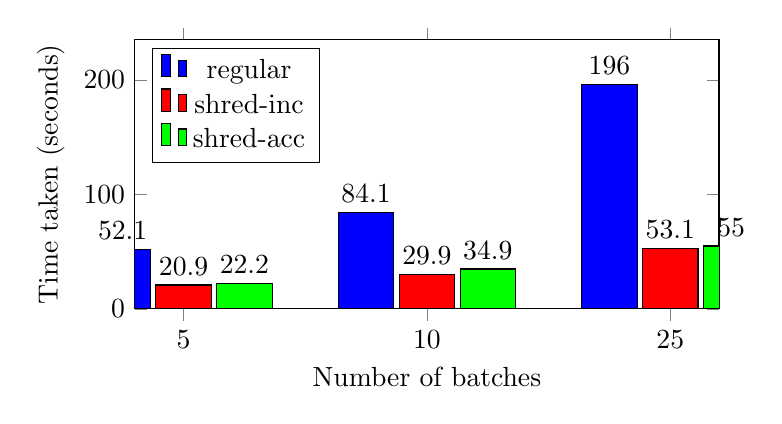
\begin{tikzpicture}
    \begin{axis}[
        ybar,
        ymin=0,
        width  = 9cm,
        height = 5cm,
        bar width=20pt,
        ylabel={Time taken (seconds)},
        xlabel={Number of batches},
        nodes near coords,
 %      nodes near coords align=below, % places labels inside bars
        symbolic x coords={5,10,25},
        xtick = data,
        xtick align=outside,
       enlarge y limits={value=0.2,upper},
        %enlarge x limits={value=0},
        legend pos=north west
    ]
    \addplot[fill=blue] coordinates {(5, 52.1) (10, 84.1) (25, 196)};
    \addplot[fill=red] coordinates {(5, 20.9) (10, 29.9) (25, 53.1)};
    \addplot[fill=green] coordinates {(5, 22.2) (10, 34.9) (25, 55)};
      \legend{regular, shred-inc, shred-acc}
    \end{axis}
\end{tikzpicture}
\end{figure}
}
	



%now enable appendix numbering format and include any appendices
%\appendix
%\chapter{DSL Codebase} \label{codebase}

\includepdf{TestPDF}
%\chapter{Queries} \label{queries}

%next line adds the Bibliography to the contents page
%\addcontentsline{toc}{chapter}{Bibliography}
%uncomment next line to change bibliography name to references
%\renewcommand{\bibname}{References}
%\bibliography{refs}        %use a bibtex bibliography file refs.bib
%\bibliographystyle{plain}  %use the plain bibliography style

\end{document}

